\documentclass[journal]{vgtc}                % final (journal style)
%\documentclass[review,journal]{vgtc}         % review (journal style)
%\documentclass[widereview]{vgtc}             % wide-spaced review
%\documentclass[preprint,journal]{vgtc}       % preprint (journal style)
%\documentclass[electronic,journal]{vgtc}     % electronic version, journal

%% Uncomment one of the lines above depending on where your paper is
%% in the conference process. ``review'' and ``widereview'' are for review
%% submission, ``preprint'' is for pre-publication, and the final version
%% doesn't use a specific qualifier. Further, ``electronic'' includes
%% hyperreferences for more convenient online viewing.

%% Please use one of the ``review'' options in combination with the
%% assigned online id (see below) ONLY if your paper uses a double blind
%% review process. Some conferences, like IEEE Vis and InfoVis, have NOT
%% in the past.

%% Please note that the use of figures other than the optional teaser is not permitted on the first page
%% of the journal version.  Figures should begin on the second page and be
%% in CMYK or Grey scale format, otherwise, colour shifting may occur
%% during the printing process.  Papers submitted with figures other than the optional teaser on the
%% first page will be refused.

%% These three lines bring in essential packages: ``mathptmx'' for Type 1
%% typefaces, ``graphicx'' for inclusion of EPS figures. and ``times''
%% for proper handling of the times font family.

\usepackage{mathptmx}
\usepackage{graphicx}
\usepackage{times}

%% We encourage the use of mathptmx for consistent usage of times font
%% throughout the proceedings. However, if you encounter conflicts
%% with other math-related packages, you may want to disable it.

%% This turns references into clickable hyperlinks.
\usepackage[bookmarks,backref=true,linkcolor=black]{hyperref} %,colorlinks
\hypersetup{
  pdfauthor = {},
  pdftitle = {},
  pdfsubject = {},
  pdfkeywords = {},
  colorlinks=true,
  linkcolor= black,
  citecolor= black,
  pageanchor=true,
  urlcolor = black,
  plainpages = false,
  linktocpage
}

%% If you are submitting a paper to a conference for review with a double
%% blind reviewing process, please replace the value ``0'' below with your
%% OnlineID. Otherwise, you may safely leave it at ``0''.
\onlineid{0}

%% declare the category of your paper, only shown in review mode


%% allow for this line if you want the electronic option to work properly


%% In preprint mode you may define your own headline.
%\preprinttext{To appear in an IEEE VGTC sponsored conference.}

%% Paper title.

\title{Visual Analytics on Credit Cards Defaults}
%\subtitle{Visual Analytics project, A.Y. 2017/2018}

%% This is how authors are specified in the journal style

%% indicate IEEE Member or Student Member in form indicated below
\author{Maria Ludovica Costagliola, Emanuele De Santis}


%other entries to be set up for journal
%\shortauthortitle{Firstauthor \MakeLowercase{\textit{et al.}}: Paper Title}

%% Abstract section.
\abstract{
The project here described was developed to put into practice all teachings
of the Visual Analytics course. It concerns the visualization of credit card
owners data in order to make a possible bank director knowing customers that
are supposed to not be able to pay their credit card bill the next month.
All data are represented using well-known views to keep the interface as
simple as possible to interact with: its structure allows to give an
overview on all customers at the same time and to immediately recognize
similarities between them.

The system relies on a machine learning algorithm to classify new customers,
that can be added from the interface using a form, and to represent them
updating all views.

} % end of abstract

%% Keywords that describe your work. Will show as 'Index Terms' in journal
%% please capitalize first letter and insert punctuation after last keyword


%% ACM Computing Classification System (CCS).
%% See <http://www.acm.org/class/1998/> for details.
%% The ``\CCScat'' command takes four arguments.


%% Uncomment below to include a teaser figure.
  \teaser{
 \centering
 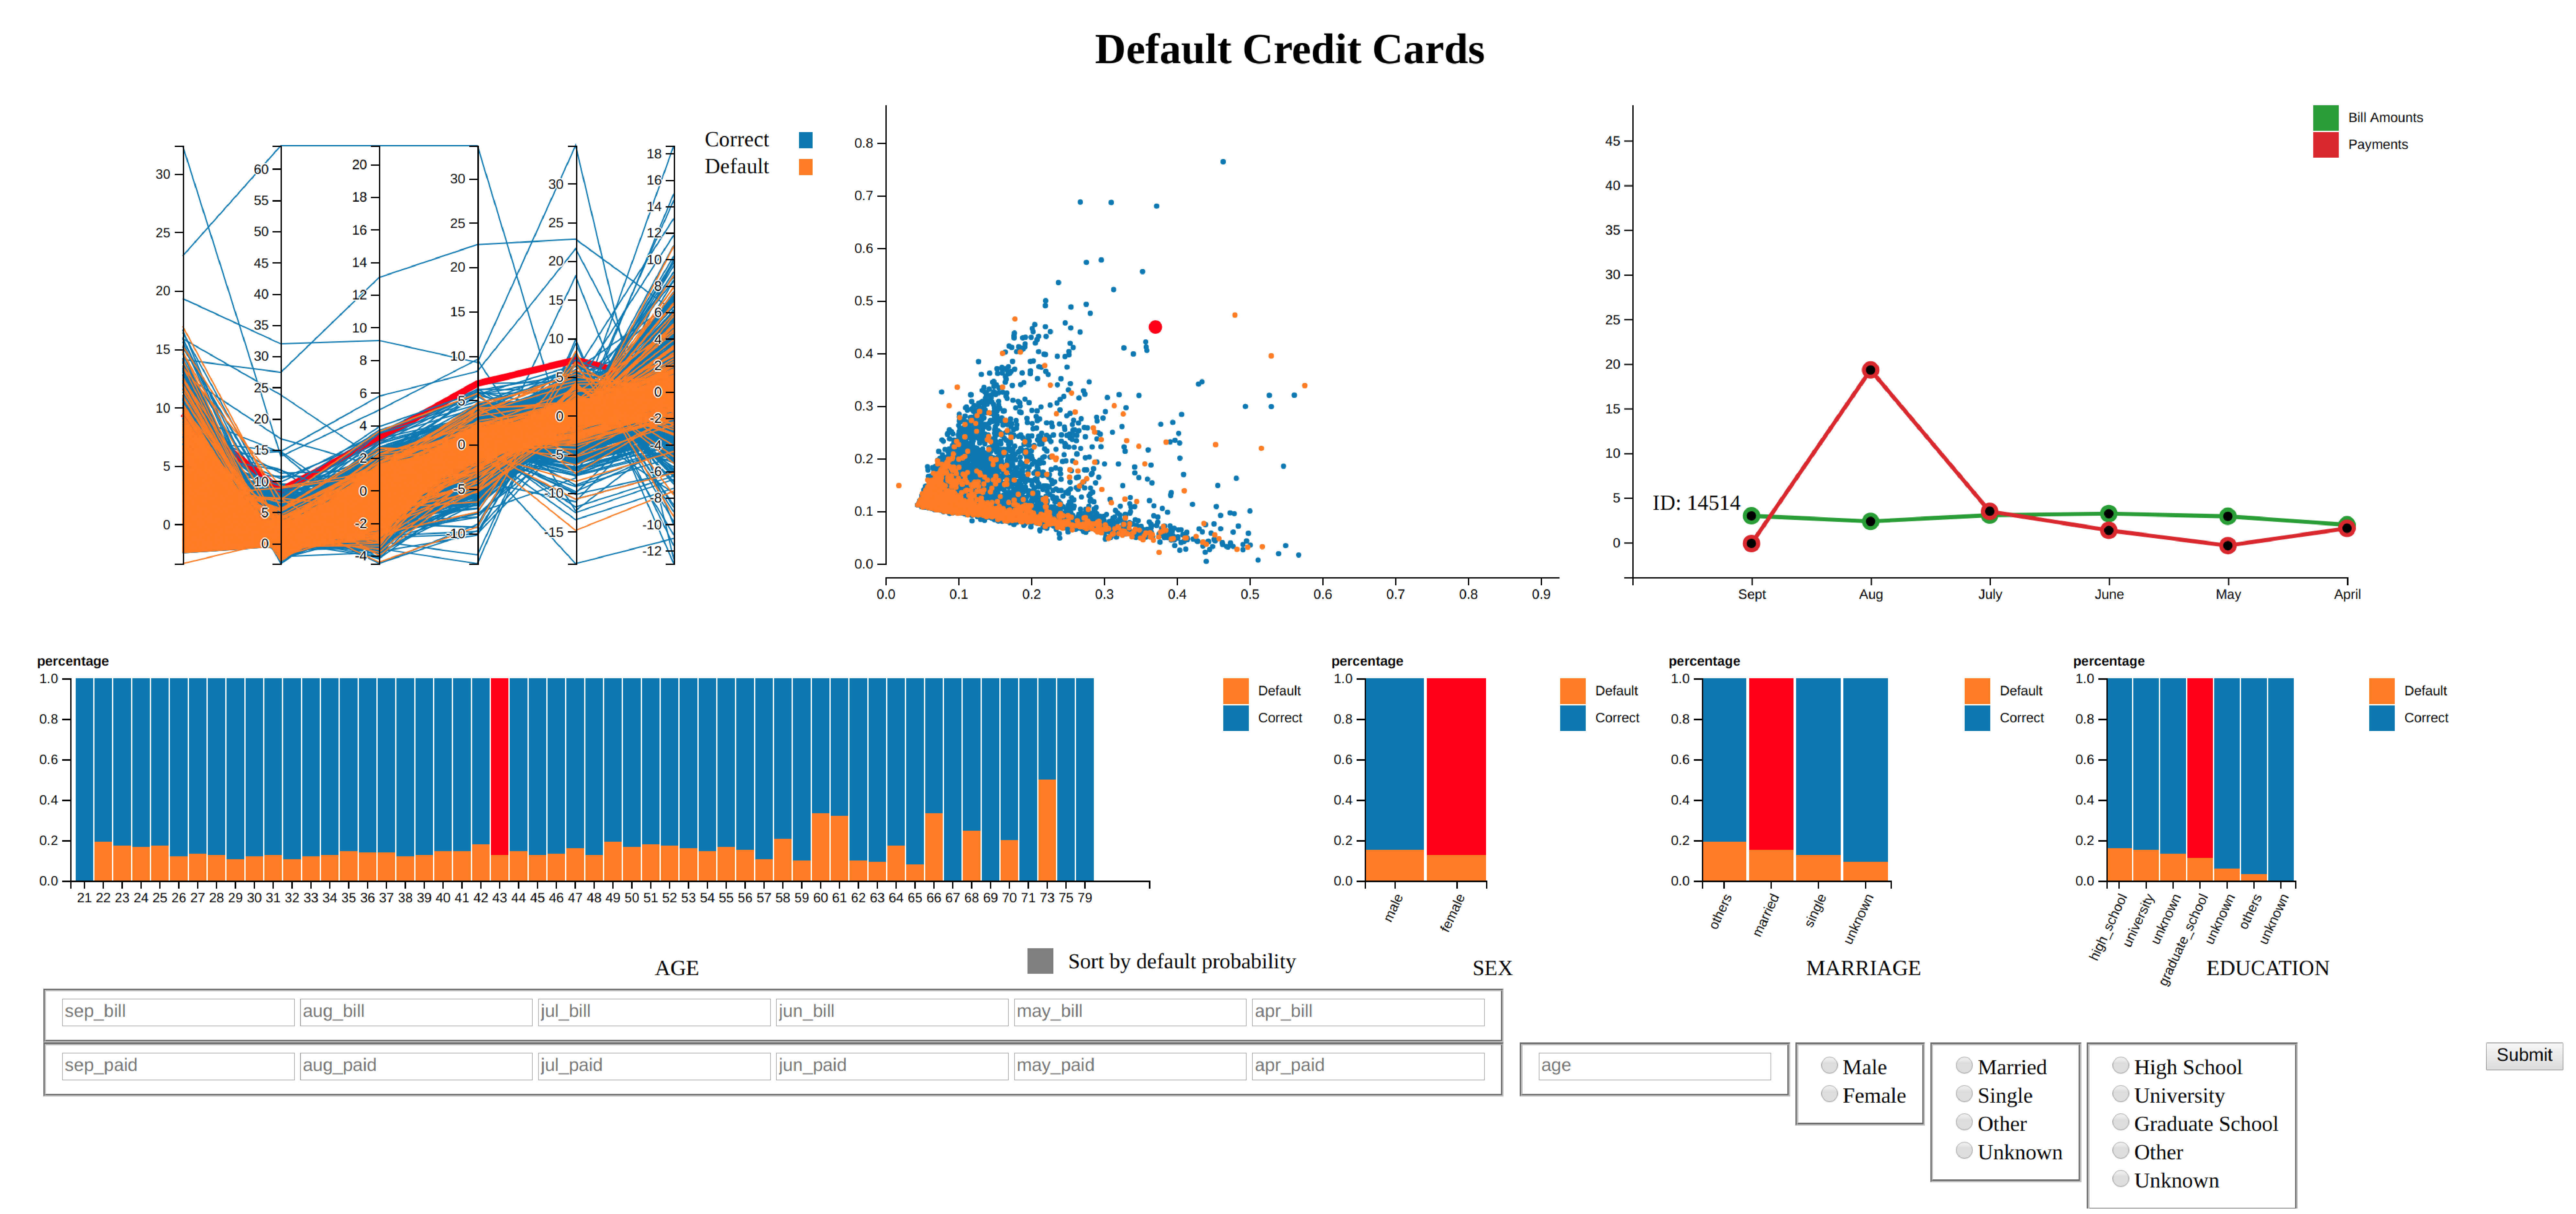
\includegraphics[width=16cm]{views}
  \caption{Sceenshot of the entire interface}
  }

%% Uncomment below to disable the manuscript note
\renewcommand{\manuscriptnotetxt}{}

%% Copyright space is enabled by default as required by guidelines.
%% It is disabled by the 'review' option or via the following command:
% \nocopyrightspace

%%%%%%%%%%%%%%%%%%%%%%%%%%%%%%%%%%%%%%%%%%%%%%%%%%%%%%%%%%%%%%%%
%%%%%%%%%%%%%%%%%%%%%% START OF THE PAPER %%%%%%%%%%%%%%%%%%%%%%
%%%%%%%%%%%%%%%%%%%%%%%%%%%%%%%%%%%%%%%%%%%%%%%%%%%%%%%%%%%%%%%%%

\begin{document}

%% The ``\maketitle'' command must be the first command after the
%% ``\begin{document}'' command. It prepares and prints the title block.

%% the only exception to this rule is the \firstsection command
\firstsection{Introduction}

\maketitle

%% \section{Introduction} %for journal use above \firstsection{..} instead

After the paper presentation done during the lectures regarding the financial
fraud detection through Visual Analytics techniques, we decided to
focus our attention on a dataset related to bank transactions.
Even though most of bank transactions datasets are not public available,
or contains just a few useful information to protect users’ privacy, we were still
able to find an interesting dataset related to this field. It represents
data about customers and their credit cards.

We were thinking about the need for a bank director to always know
how customers with a credit card issued by his financial institution
behave. Particularly, we pay attention to the last payments done by customers
and to their corresponding bank account balances.

From these data and from some other personal information of the customer (for example age, marriage status, ...), it is possible to identify the ones that probably will not be able
to pay the credit card bill in the next month.

The prediction is done by a machine learning algorithm, but the
result is useless if it is not combined with an efficient visualization
of the whole dataset. In fact, with the visualization we tought of,
a bank director is able to better understand the result of the machine
learning algorithm, considering also the similarity between the result
and some preexisting patterns or clusters.

Moreover the bank director may be able to detect default customers even without using any machine learning algorithm, just seeing the information given by the visualization.


\section{Dataset}
The dataset used in this project is taken from UCI database \cite{UCI:2016} , it contains about 30000 tuples, each with 24 attributes.
Some tuples lack of some values and so they were all removed in order to have a completely useful dataset. A few attributes for each remaining tuple were also removed because they were of no interest for us. We get in this way a more manageable dataset thanks to a lower number of tuples (15337) and of attributes (19).
This computation was done by the python function \texttt{preprocessing.action()}, that creates a new csv file named \texttt{dataset.csv}.

About the used attributes, we can identify four of them that are categorical: age, sex, marriage status, education. These represent personal information about the owner of a particular credit card and they are used for statistical considerations. We have six numerical attributes named \textit{Amount of bill statement}, one for each month from September 2005 to April 2005 and the corresponding six numerical, named \textit{Amount of previous payment}.

The last attribute of each row is the \textit{target}, that is the prediction about the ability to pay on October 2005.


\section{Visualization}
The visualization that we have developed is constituted by 7 views,
each one that shows different aspects of the dataset.

All of them are coordinated each other, so clicking on an element of a
certain view, the event handler will highlight some elements in the
others and/or will show other information. Moreover when a new customer
is added, all views change according to the newly added tuple.

The interface was tought to fit in a FullHD (1920x1080) screen,
even if it works also if we resize the browser window (the minimun
resolution supported is 1024x768).


\subsection{Scatterplot}

\begin{figure}[h]
  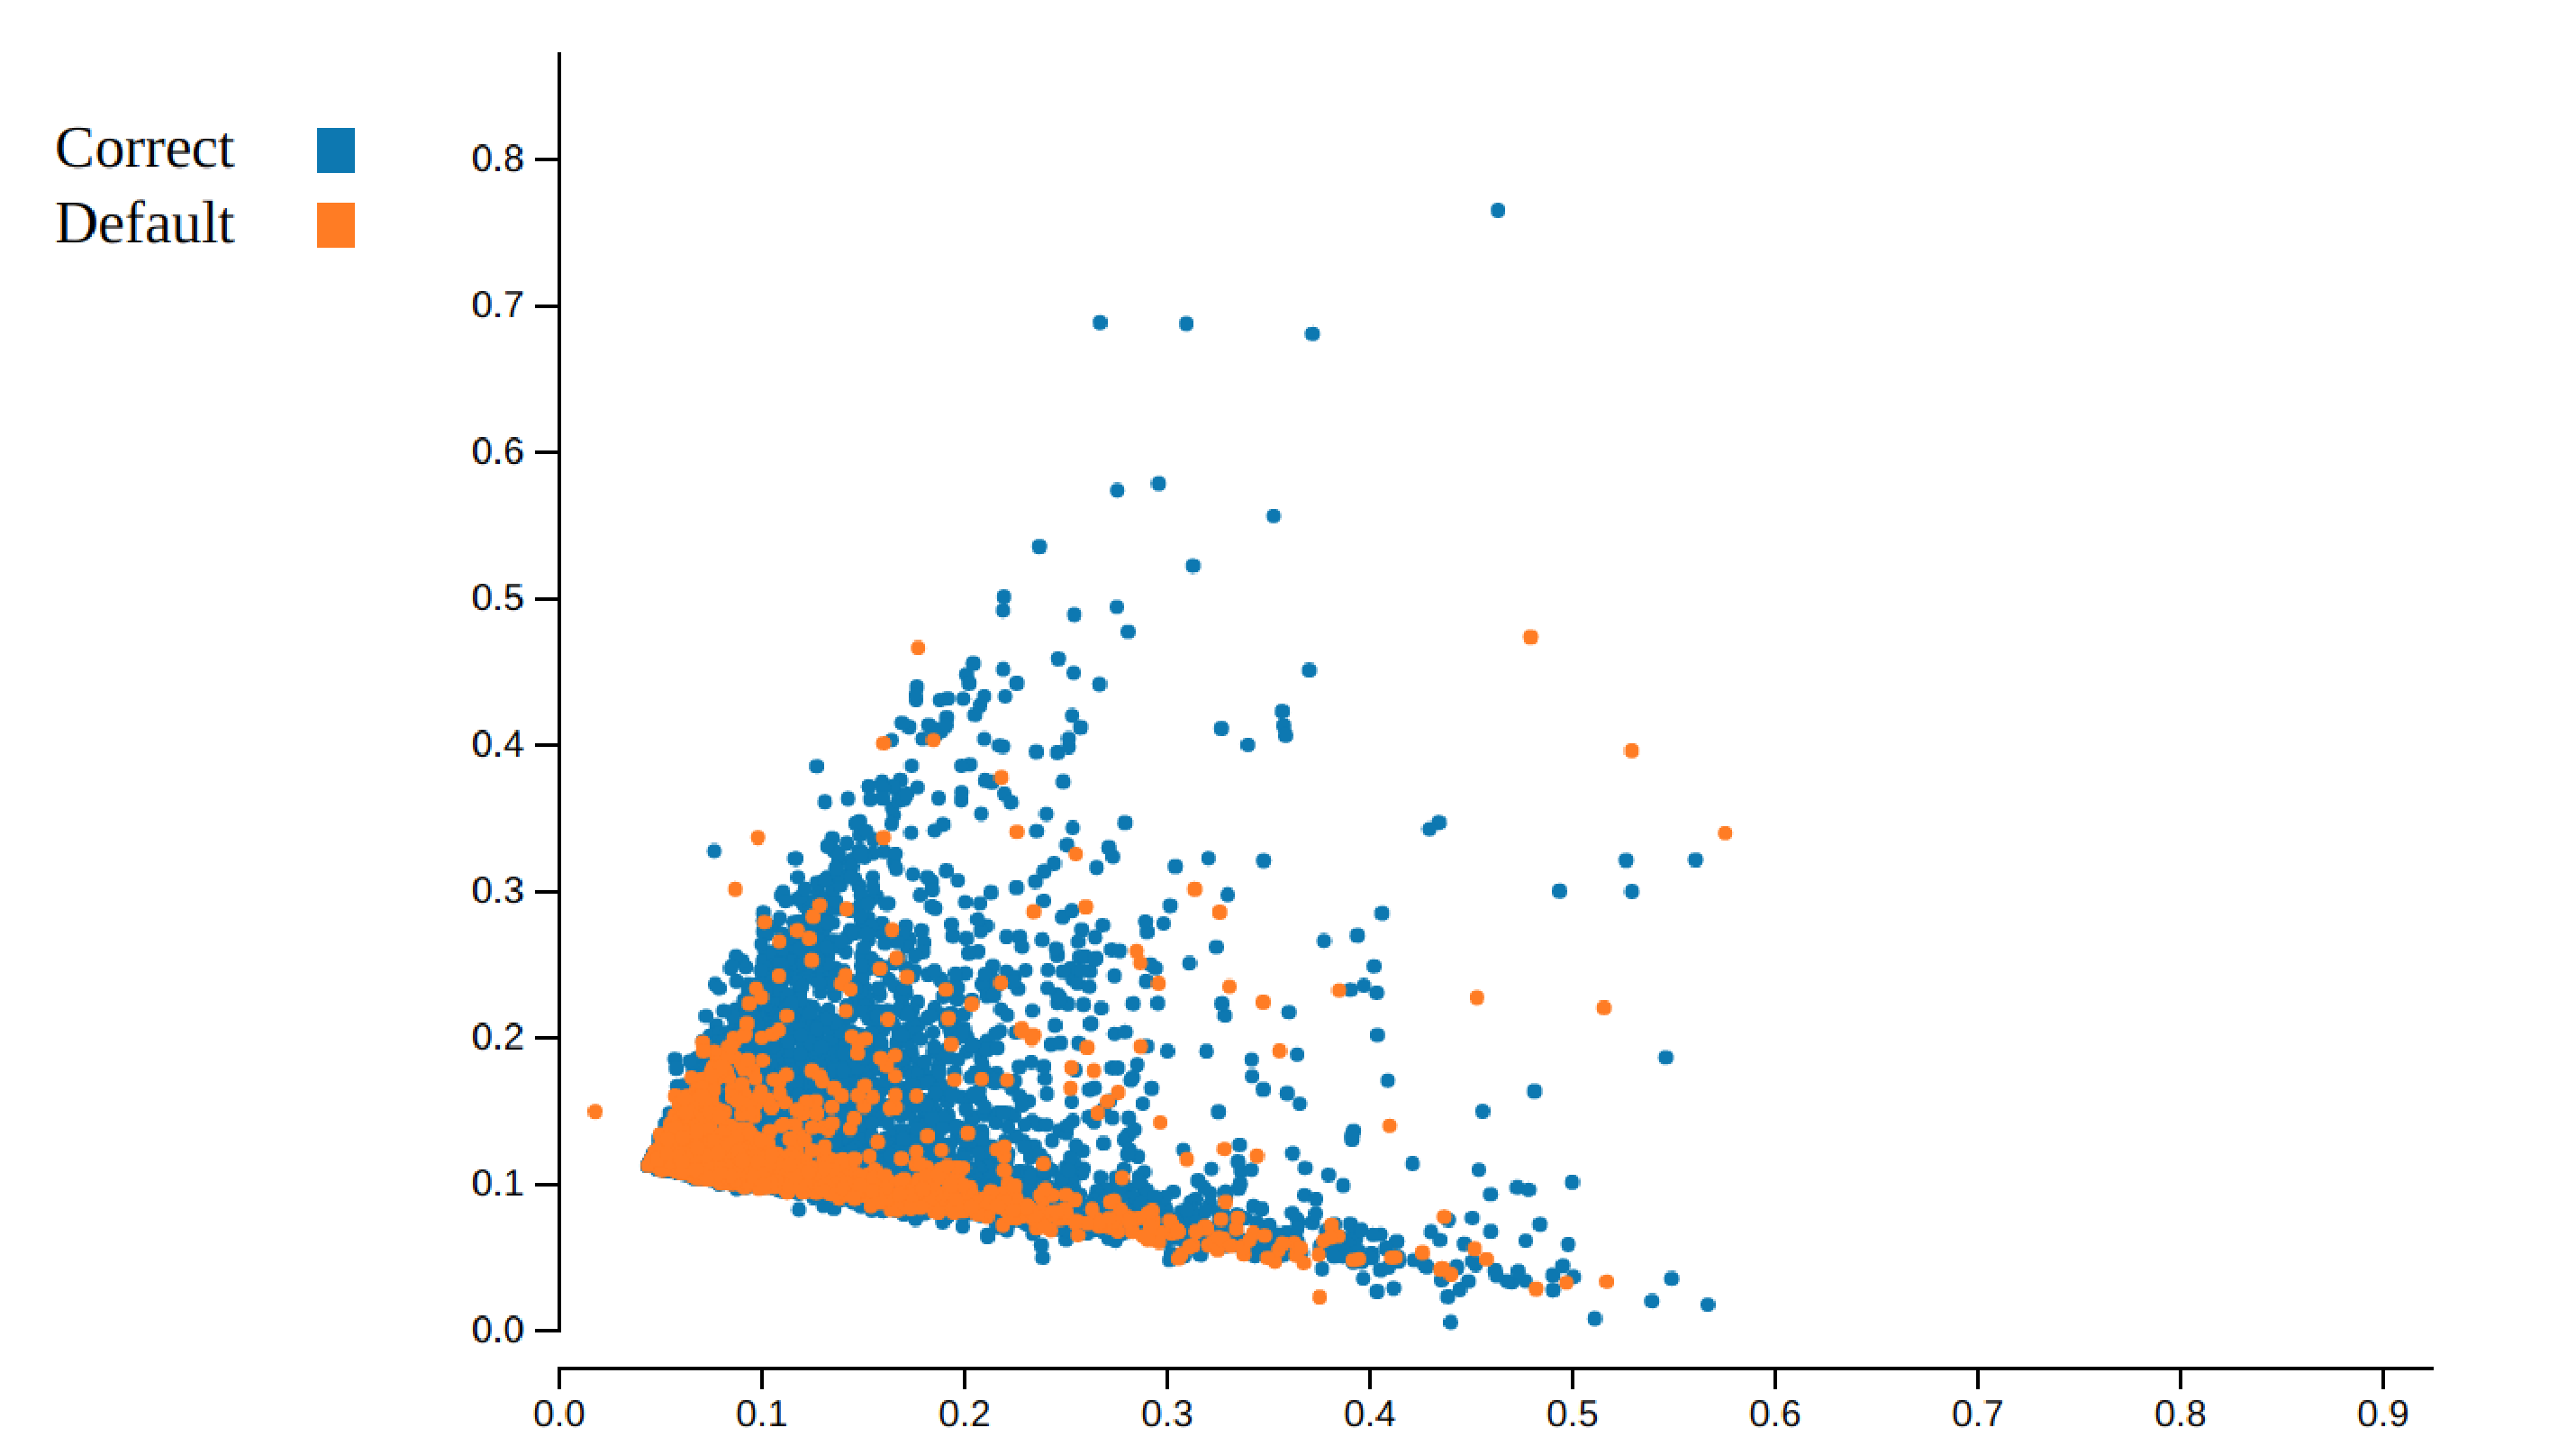
\includegraphics[scale=0.15]{scatterplot}
  \caption{Scatterplot view of the tool}
  \label{scatterplot}
\end{figure}
The scatterplot is the main view in the visualization. Each point represents a customer and the color encodes the classification of the customer (default or correct). The color scaling used is the \texttt{d3.scaleOrdinal(d3.schemeCategory10)}.

Due to the high dimensionality of the dataset, it was mandatory to apply a dimensionality reduction algorithm. We decided to apply PCA because it is fast and it doesn't require a deep knowledge of the problem, and we then took the first 2 components. This work is done by the python function \texttt{pca.action()} using \texttt{pandas} to read and parse the csv original dataset
and \texttt{sklearn} to compute PCA values. The result is saved in \texttt{pca.csv}.

A 2D scatterplot is the best way to graphically represent the relation between points and to spot possible clusters. In this case it helps the bank director to quickly see that most of the bad customers are grouped together in a particular area (in figure \ref{scatterplot} in the left-bottom part of the plot).

Each point has associated two event handlers. The first one allows to make visible a tooltip showing the identifier of the customer just by mouseovering over it; this handler also makes the point bigger to have it more visible.
The second handler is associated to click events: by clicking on a point, it will highlight the point itself, will trigger the highlighting of all other related elements and will show up the corresponding lines in the linechart.

Associated to the scatterplot is present a legend explaining the color encoding and clicking on an element of the legend, it is possible to see on the foreground all the points with that classification. Once an element is clicked, a reset button appears in order to
restore the original view.

\subsection{Parallel Coordinates}
\begin{figure}[h]
  \centering
  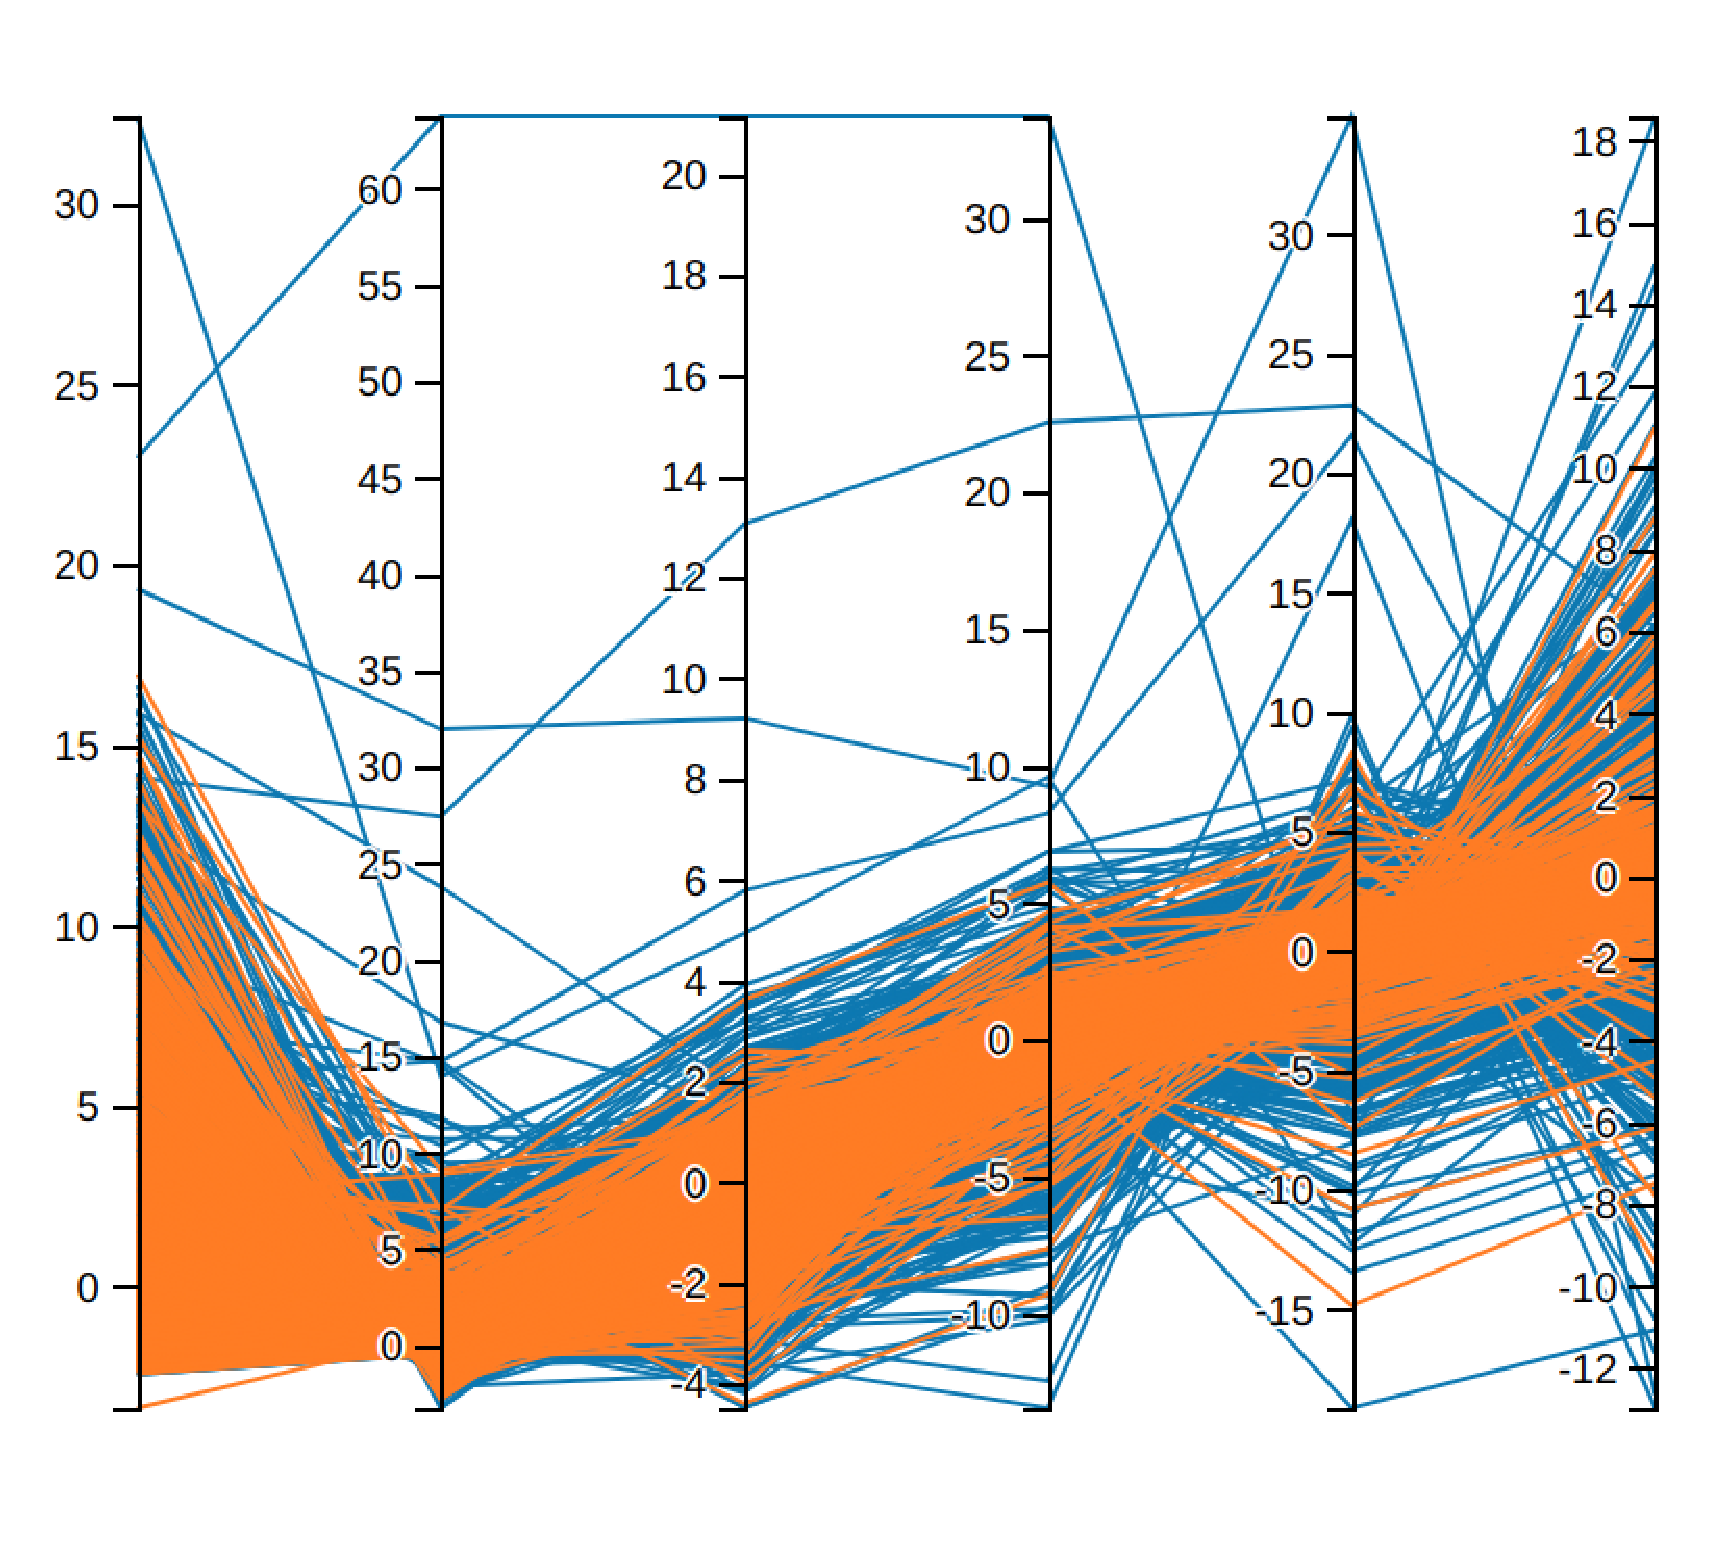
\includegraphics[scale=0.15]{parallel}
  \caption{Parallel Coordinates view of the tool}
  \label{parallel}
\end{figure}

Parallel Coordinate view is an efficient way to represent data with more than 2 dimensions in a 2D space. Moreover it allows to grasp relations between tuples (for example crossing lines may correspond to a linear relation on some axis).

We have six axis, that correspond to the first
six principal components given by the PCA algorithm applied on the original dataset (\texttt{dataset.csv}). Each line referrs to one single point that is the
graphic representation of a customer. Also in this case we use the same color encoding as before to distinguish between default and correct customers.

There is the possiblilty to click on a line to select it and to see the corresponding point in the scatterplot highlighted together with all the related information (having the same behaviour we had by clicking on a point in the scatterplot)

Moreover it is possible to exchange the order of the axis, dragging the axis that we want to move. Unfortunately, since the dataset contains a lot of tuples, the movement is a little bit glitchy.


\subsection{Linechart}

\begin{figure}[h]
  \centering
  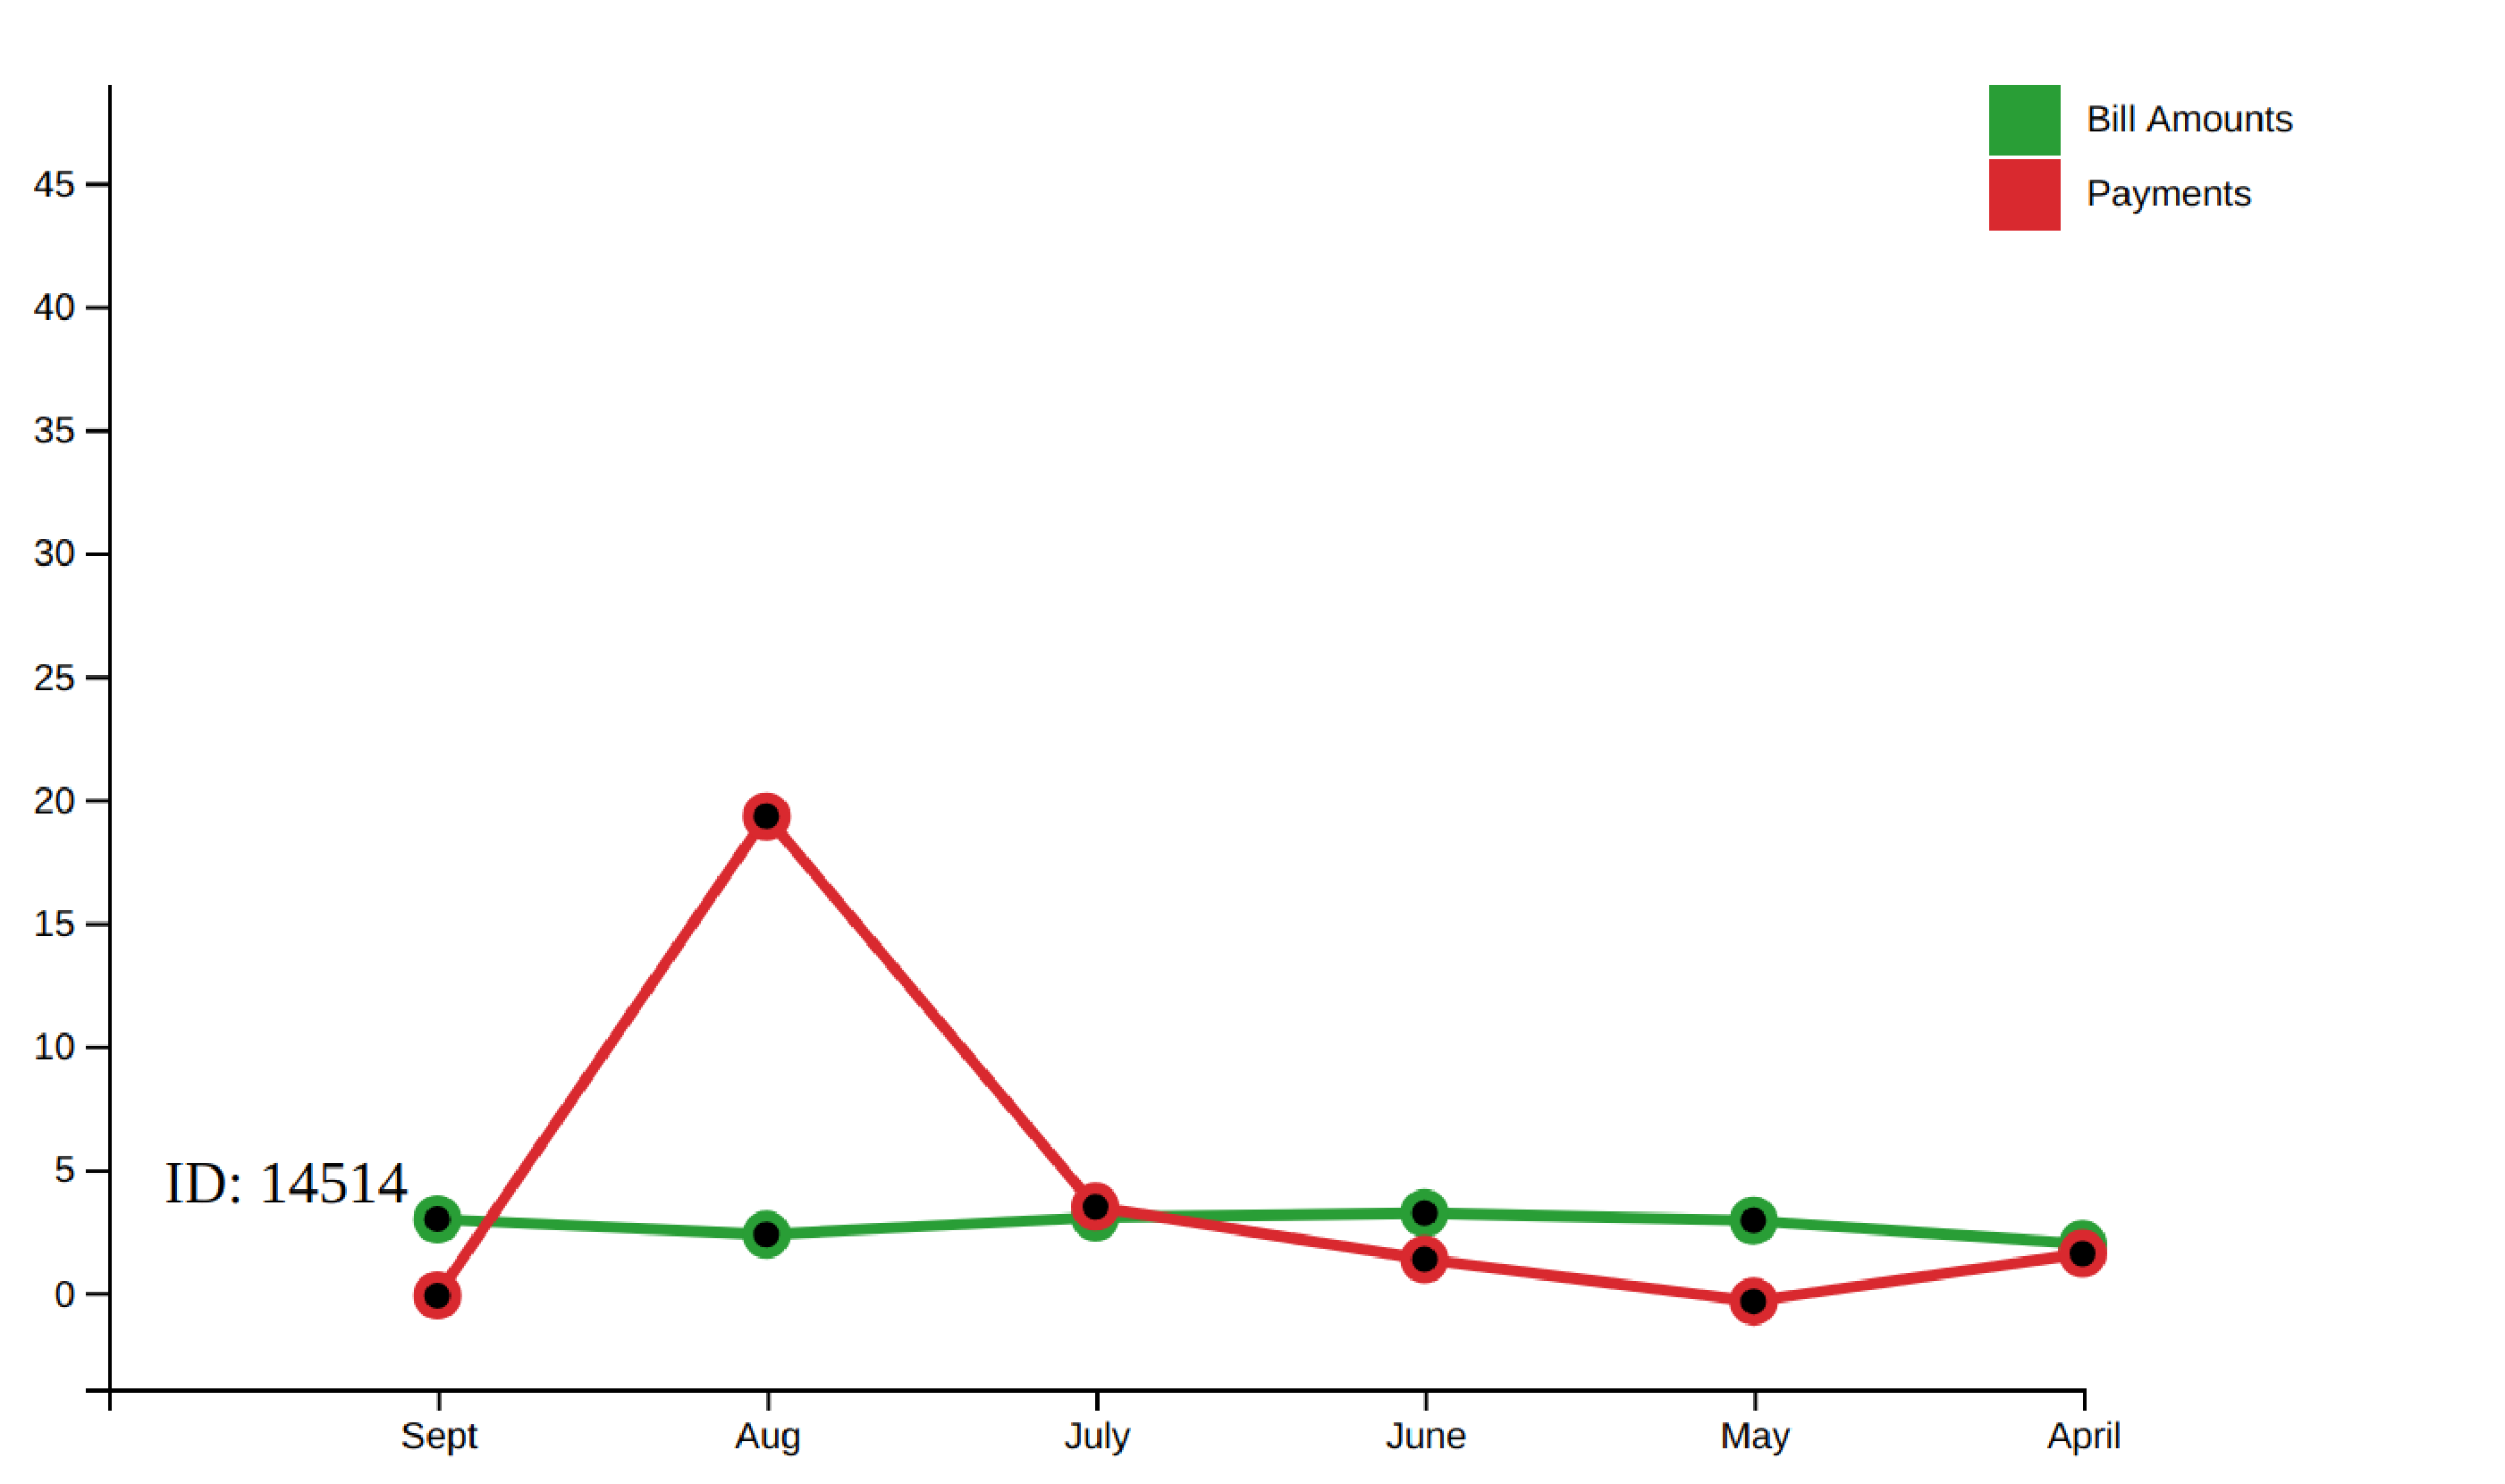
\includegraphics[scale=0.15]{linechart}
  \caption{Linechart view of the tool}
  \label{linechart}
\end{figure}

Each customer has associated some numerical values that refer to a specific month. We decided to use a line chart to represent these attributes since they are temporal related data.

We can distinguish two lines: the green one represents the amount of money the customer had in his bank account in the specified period, while the red one represents the payments that he did
with his credit card.

The values that are represented are often not of the same order of magnitude, so we had to compute a normalized version of the dataset (saved in \texttt{standardized\_data.csv}) using \texttt{Standardization.action()} function, that applies
a \texttt{numpy} standard scaler to all these amounts.

On the plot is also written the ID of the displayed customer and, since the values are normalized, we thought it could be useful to retrieve the original amounts in some way. In fact on each line there are 6 circles that can be mouseovered in orderd to see in a tooltip
the original value of that point, while on the y-axis are represented the normalized values.

As soon as the page is loaded this view is empty and will be filled with the information described and with a legend of the color used once a point in the scatterplot or a line in the parallel coordinates is selected.

\subsection{Stacked Barcharts}
\begin{figure}[h]
  \centering
  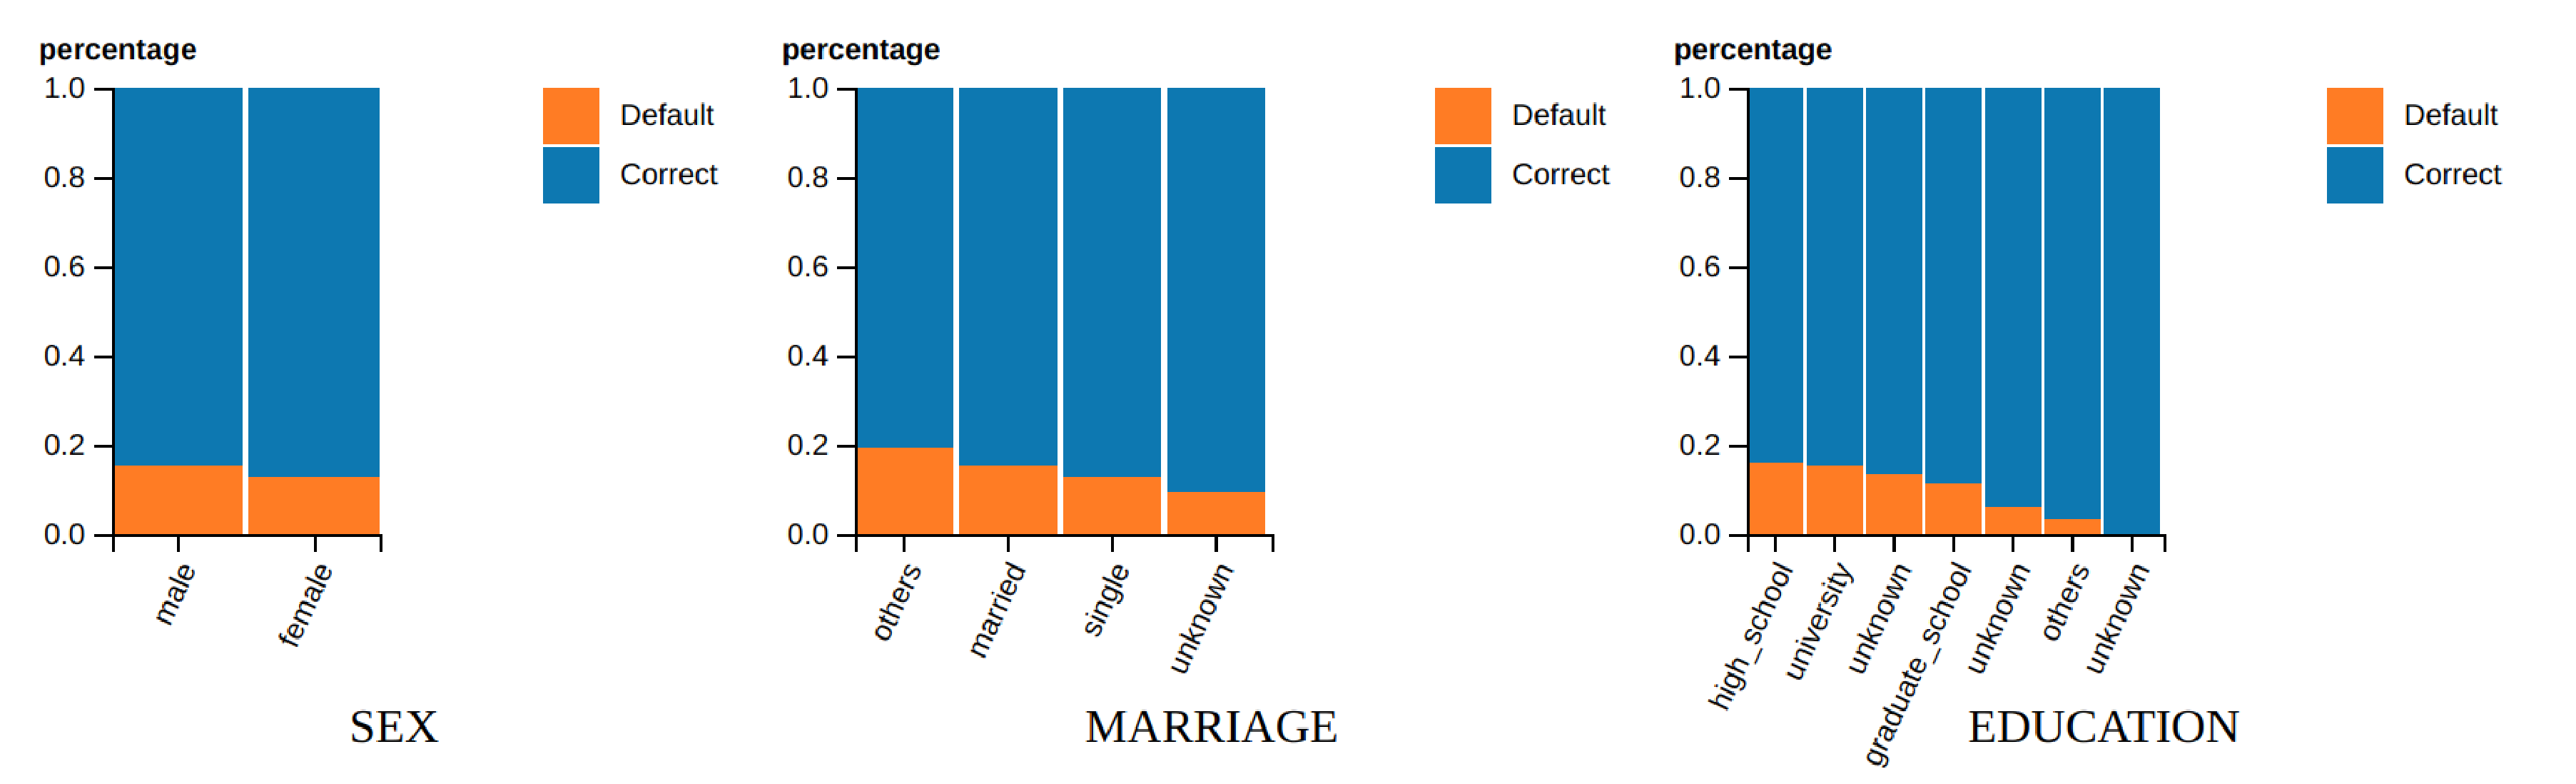
\includegraphics[scale=0.15]{stacked}
  \caption{Stacked Barcharts representing frequency distributions of the categorical attributes sex, marriage and education}
  \label{stacked}
\end{figure}

Each categorical attribute of the dataset is represented through a stacked barchart. This kind of visualization allows us to see at the same time the frequency distribution of both correct and default customers.
There is one column for each different value of the categorical attribute, composed by two sub-columns. Each of those represents the percentage of default (on the bottom) and of correct (on the top) instances in the dataset.
These data are taken from \texttt{*\_frequency.csv}.

We added some interactions with this chart. First of all, the element of the legend can be clicked in order to see only the frequency of the chosen classification;
after this interaction, it spawns a reset button to restore the original view.

A tooltip shows up mouseovering over a single bar; it contains the number of instances, taken from \texttt{*\_instances.csv}, within its classification and its value for the attribute in exam. We decided to use a tooltip since the height of some bars
can be very small, so a number inside them could not be clearly visible or it could overflow into the bars close to it.

Finally, each bar can be clicked: it will be highlighted together with all points in the scatterplot and lines in the parallel coordinates that correspond to customers
that have the same value for the attribute and the corresponding classification of the clicked bar.

Once the user clicks on a point in the scatterplot or on a line in the parallel coordinates, the bars, that correspond to the value of the respective attribute for the selected customer, are highlighted in each stacked barchart.

The columns of all the stacked barcharts (except for the Age one) are sorted according to the percentage of default accounts, to improve visibility of categories of people that are more at risk to be default customers; for the same
reason we choose to put the default percentage at the bottom of the stack.

\subsubsection{Stacked Barchart: Age}
\begin{figure}[h]
  \centering
  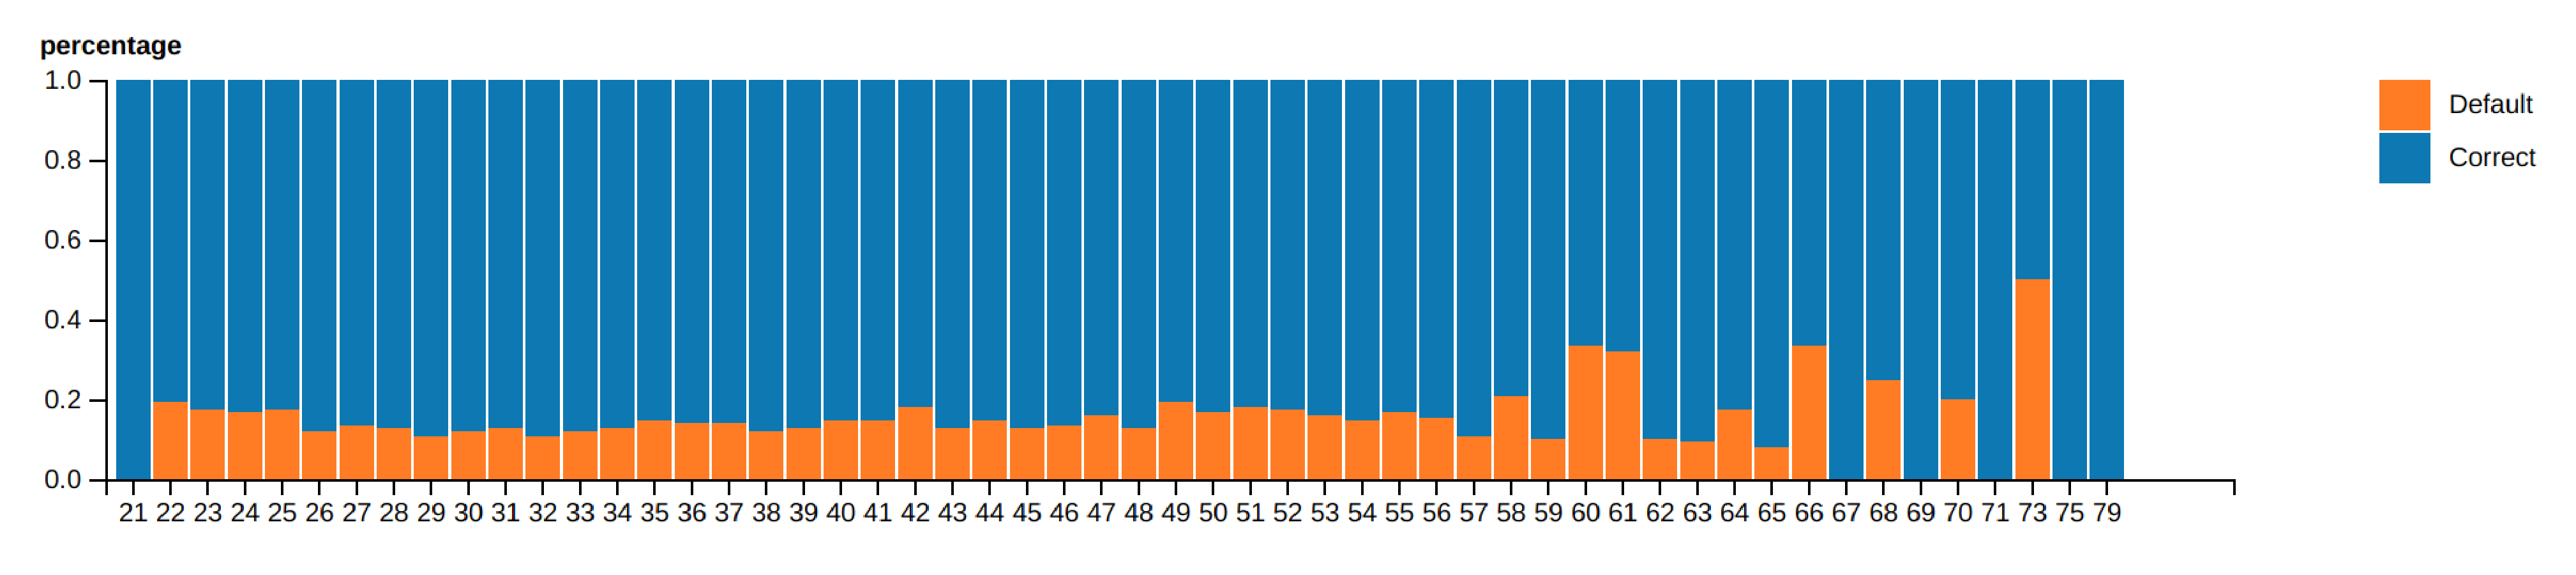
\includegraphics[scale=0.13]{age}
  \caption{Stacked Barchart representing frequency distribution of ages}
  \label{age}
\end{figure}

This stacked barchart corresponding to the age behaves in the same way of the others, but it contains something more.
Ages have a natural intrinsic order and so, by default, the columns are sorted in that way, but we added the possibility
to change the order and have them sorted according to the default percentage.

To make this happen there is a button \texttt{Sort by default percentage} to click, the columns will change their order and
the button will now permit to go back to the original sorting by age.

\subsection{New Data Form}
\begin{figure}[h]
  \centering
  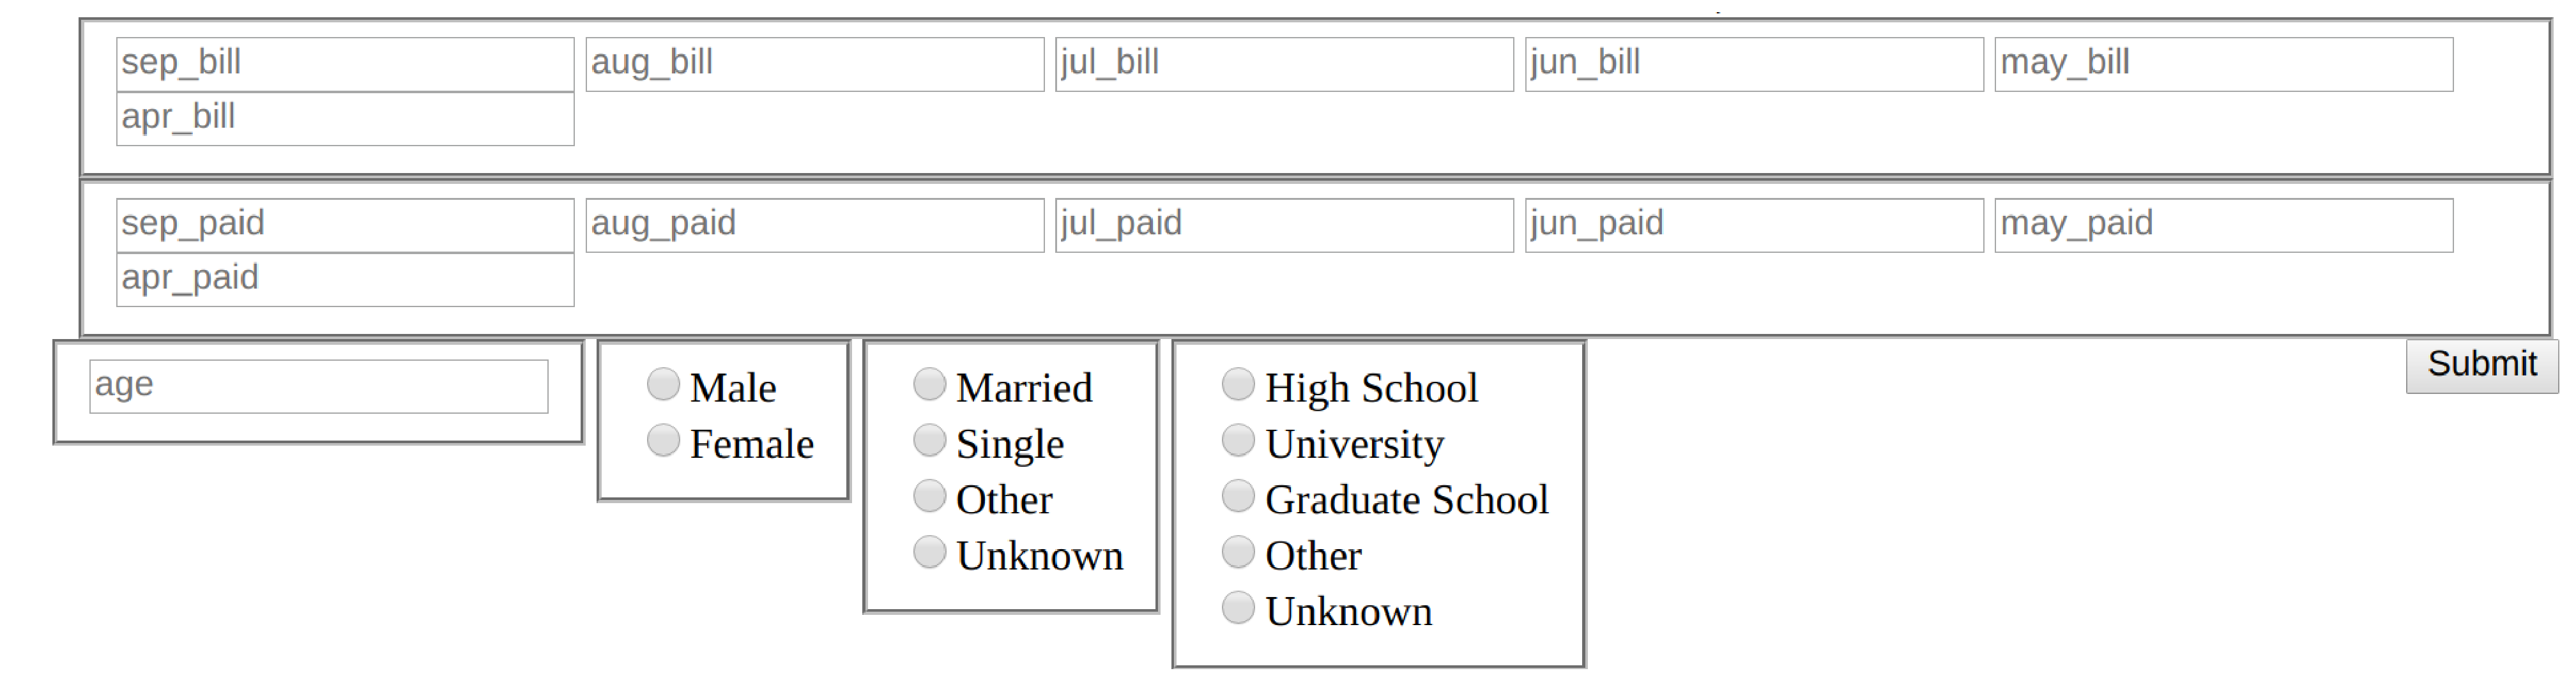
\includegraphics[scale=0.1]{form}
  \caption{Form used to add new instances to the dataset}
  \label{form}
\end{figure}


We thought about the possibility to add a new instance to the dataset. The bank director could be interested to know if a customer that is not in the dataset with certain attributes values
will be in default or correct.

Through this form, he will insert all the values associated to this new instance. Submitting them, the new tuple will be classified
using a machine learning algorithm. The browser page will be reloaded and the new point highlighted in the scatterplot.

\section{Analytics}

As said before, it is important to let an user insert new instances, but these insertions have to be reflected on the entire interface, that has to be updated according to the new data.
Moreover each new instance need to be classified to be correctly represented in the visualization and to update the frequency distributions.

Since Javascript is not so fast handling large amount of data and it is not suitable doing intense computations, we needed to move the analytics part into a python program.

To do so, we set up a small web server using the python library \texttt{flask} (that runs locally on our machines) that can communicate with the visualization.

The visualization can be accessed after the server is started at the address \texttt{http://127.0.0.1:5000} (or \texttt{http://localhost:5000}). It is now possible to pass every field value of the form
using AJAX call. AJAX sends an HTTP POST message to a fixed route of our web server, that contains a JSON payload that includes all fields.

As soon as the web server is started, it starts training an SVM learner with all the pre-classified instances present in the original dataset (\texttt{dataset.csv}).
SVM (Support Vector Machine) \cite{Boser:1992:TAO:130385.130401} is a machine learning algorithm that tries to find an hyperplain that maximizes the margin between itself and the closest points in the high dimensional space (these points are called \textit{support vectors}). In this case
SVM works on a kernelized space with an \textit{rbf} kernel (Radial Basis Function), since the dataset is not linearly separable.
We allow a certain soft margin where points can be misclassified around the classification hyperplane setting the \textit{C} parameter to 1.

If an user wants to know the accuracy of the classifier, he can run the server putting the last parameter to 1, that makes the python program compute a 3-fold cross validation on the trained algorithm. Using this dataset we reached an accuracy of 86\%.

Once the web server receives the HTTP POST message from the Javascript code, it creates a new tuple to be added to \texttt{dataset.csv} and it classifies it using the pre-trained SVM classifier. The new line is appended, and then the function calls all our python modules,
 that will re-compute all additional csv files (for example \texttt{*\_frequency.csv} and \texttt{*\_instances.csv}), required by the interface.


At the end of the computation it returns to the Javascript code the ID associated to the newly added customer.
At this point Javascript can make an alert message showing the ID returned and can highlight the point associated to this ID in the scatterplot.

\section{Conclusion}

In this work we presented an intuitive tool that can be used in a financial institution to monitor the behaviour of the customers that have a credit card issued by the financial institution itself. It can be also useful in case
the bank director has to decide to issue a new credit card to one of his customers, knowing the spending patterns and the bank account bills of that customer.

The power of this tool is that it combines both machine learning and visual analytics methodologies, so a bank director can classify new instances using SVM classifier and validate the classification done using the visualization, and can also make a prediction
without any use of machine learning algorithms, just comparing the new customer with similar ones yet present in the dataset, using all views presented here.

Due to the high number of tuples present in the dataset, the visualization is a little bit crowded; in fact a lot of the visual elements presented do not scale very well as the number of tuples to be visualized increases. At the same time the SVM classifier is
very well trained since we have a lot of samples (it reaches the accuracy of 86\% with half of the original dataset from \cite{UCI:2016}).

The high number of tuples makes also the interaction with the visualization a little bit glitchy but the latency experienced is still acceptable.


\bibliographystyle{abbrv}
%%use following if all content of bibtex file should be shown
%\nocite{*}
\bibliography{template}
\end{document}
